\chapter{Classificação de Tipo de Superfície de Pista 2}
\label{cap:classificacao_tipo_superficie_2}

Através dos resultados obtidos no estudo da seção anterior, foi conduzido um segundo estudo para o desenvolvimento de modelo adaptativo de classificação de tipo de superfície de pista, com foco em modelos de \textit{Deep Learning}, os quais se mostraram mais promissores quando comparados a modelos de Aprendizado de Máquina clássicos. Neste estudo foi produzido em conjunto uma avaliação multiaspecto e multicontextual. O processo de desenvolvimento e experimentação é detalhado nas próximas subseções. Na primeira delas, o pré-processamento, os dados foram ajustados e organizados para avaliar aspectos como a influência do ponto de coleta de dados no veículo, o domínio de análise, as características de entrada do modelo e o tamanho da janela de dados. Também foi avaliada a capacidade de generalização do aprendizado dos modelos para contextos desconhecidos. Na segunda subseção, processamento, foram desenvolvidos três modelos de DNN baseados em diferentes técnicas de \textit{Deep Learning}: LSTM, GRU e CNN. Por fim, na última subseção são detalhados e comparados os resultados obtidos.

\section{Pré-Processamento}

Na etapa de pré-processamento os dados foram organizados e transformados para serem utilizados como entrada dos modelos de classificação. Esta etapa incluiu a separação de dados para treinamento e validação do modelo, a definição das características de entrada, a normalização dos dados das características e o agrupamento de dados em janelas. Neste estudo, foram utilizados os dados de aceleração em três eixos (X, Y, Z) e em três pontos de coleta diferentes (abaixo e próximo da suspensão, acima e próximo da suspensão e no painel de controle), juntamente com a taxa de rotação em três eixos e nos três pontos de coleta, além da velocidade do veículo.

Com o objetivo de avaliar a influência da propriedade de dependência veicular e verificar a viabilidade de um modelo de classificação para os dados coletados em diferentes locais do veículo, definimos os seguintes \emph{experimentos por colocação}, com base nos pontos de coleta de dados no veículo:

\begin{description}
	
	\item[Experimento por Colocação 1:] Foram utilizados os dados de força de aceleração 3D e taxa de rotação 3D amostrados próximo e abaixo da suspensão, mais a velocidade.
    
    \item[Experimento por Colocação 2:] Foram utilizados os dados de força de aceleração 3D e taxa de rotação 3D amostrados próximo e acima da suspensão, mais a velocidade.
    
    \item[Experimento por Colocação 3:] Foram utilizados os dados de força de aceleração 3D e taxa de rotação 3D amostrados no painel de controle, mais a velocidade.
    
\end{description}

Neste estudo, buscou-se identificar também o domínio de análise mais adequado para classificar o tipo de superfície de pista. Sendo assim, para cada \emph{experimento de colocação}, foram definidos \emph{experimentos por domínio de análise}. Para a análise no domínio da frequência, foram aplicados nos dados a Transformada de Fourier de Curto Tempo (\textit{Short-Time Fourier Transform} - STFT) para extrair as características de magnitude da frequência através de uma janela deslizante de 100 amostras com total sobreposição. Os \emph{experimentos por domínio de análise} foram definidos de acordo com as características de entrada detalhadas abaixo:

\begin{description}

    \item[Experimento por Domínio de Análise 1:] Foram utilizadas as 7 características correspondentes a aceleração nos eixos X, Y, Z; a taxa de rotação nos eixos X, Y, Z; e a velocidade.
    
    \item[Experimento por Domínio de Análise 2:] Foram utilizadas as 7 características do \emph{Experimento por Domínio de Análise 1}, mais quatro características de aceleração composta XY, YZ, XZ, XYZ, de acordo com as fórmulas detalhadas em \cite{Tan2019}.
    
    \item[Experimento por Domínio de Análise 3:] Foram utilizadas 357 características correspondentes às magnitudes das 51 frequências de cada uma das 7 características definidas no domínio do tempo em \emph{Experimento por Domínio de Análise 1}.
    
    \item[Experimento por Domínio de Análise 4:] Foram utilizadas 561 características correspondentes às magnitudes das 51 frequências de cada uma das 11 características definidas no domínio do tempo em \emph{Experimento por Domínio de Análise 2}.
    
\end{description}

Após definir os \emph{experimentos por domínio de análise}, os dados foram normalizados usando \textit{Min Max Scaler}. Os dados das características no domínio do tempo foram normalizados na faixa de [-1,1], uma vez que o sinal, neste caso, contém informações importantes, denotando a direção do vetor força. No domínio da frequência, como a magnitude não apresenta valores negativos, os dados foram normalizados na faixa de [0,1]. Em seguida, foram definidos os dados a serem usados no treinamento e na validação dos modelos. Para avaliar corretamente a generalização do aprendizado de cada técnica, avaliando sua adaptabilidade para contextos desconhecidos onde há variação nas propriedades de dependência veicular, de condução e ambiental, os dados de treinamento e validação foram divididos da mesma maneira que no estudo da seção anterior, separando-os de acordo com o conjunto de dados em três \emph{experimentos por contexto}:

\begin{description}
	
	\item[Experimento por Contexto 1:] O modelo aprende dados de todos os veículos e motoristas para alguns cenários; mas não todos os veículos com todos os motoristas para todos os cenários.
    \begin{itemize}
        \item \textbf{Treinamento (65\%):} PVS 1, PVS 3, PVS 4, PVS 6, PVS 7, PVS 9. 
        \item \textbf{Validação (35\%):} PVS 2, PVS 5, PVS 8.
    \end{itemize}
    
    \item[Experimento por Contexto 2:] O modelo aprende dados de todos os cenários para alguns veículos e alguns motoristas; mas não todos os veículos com todos os motoristas para todos os cenários.
    \begin{itemize}
        \item \textbf{Treinamento (66\%):} PVS 1, PVS 2, PVS 3, PVS 7, PVS 8, PVS 9.
        \item \textbf{Validação (34\%):} PVS 4, PVS 5, PVS 6.
    \end{itemize}
    
    \item[Experimento por Contexto 3:] O modelo aprende dados de alguns veículos com alguns motoristas para alguns cenários; mas não todos os veículos com todos os motoristas para todos os cenários.
    \begin{itemize}
        \item \textbf{Treinamento (66\%):} PVS 1, PVS 2, PVS 4, PVS 6, PVS 8, PVS 9.
        \item \textbf{Validação (34\%):} PVS 3, PVS 5, PVS 7.
    \end{itemize}
    
\end{description}

Finalmente, para analisar a influência do número de amostras na classificação, foram criados três \emph{experimentos por tamanho de janela de dados}, com janelas de 100, 200 e 300 amostras. A janela de dados utilizada foi fixa sem sobreposição, e cada amostra correspondeu a um vetor com os valores das características. Em resumo, cada experimento realizado neste estudo é um elemento do produto cartesiano entre \emph{experimentos por colocação}, \emph{experimentos por domínio de análise}, \emph{experimentos por contexto} e \emph{experimentos por tamanho de janela de dados}, conforme ilustra a \autoref{fig:combinacao_experimentos_2}.

\begin{figure}[h!]
  \centering
  \caption{Combinação de tipos de experimentos}
  \label{fig:combinacao_experimentos_2}
  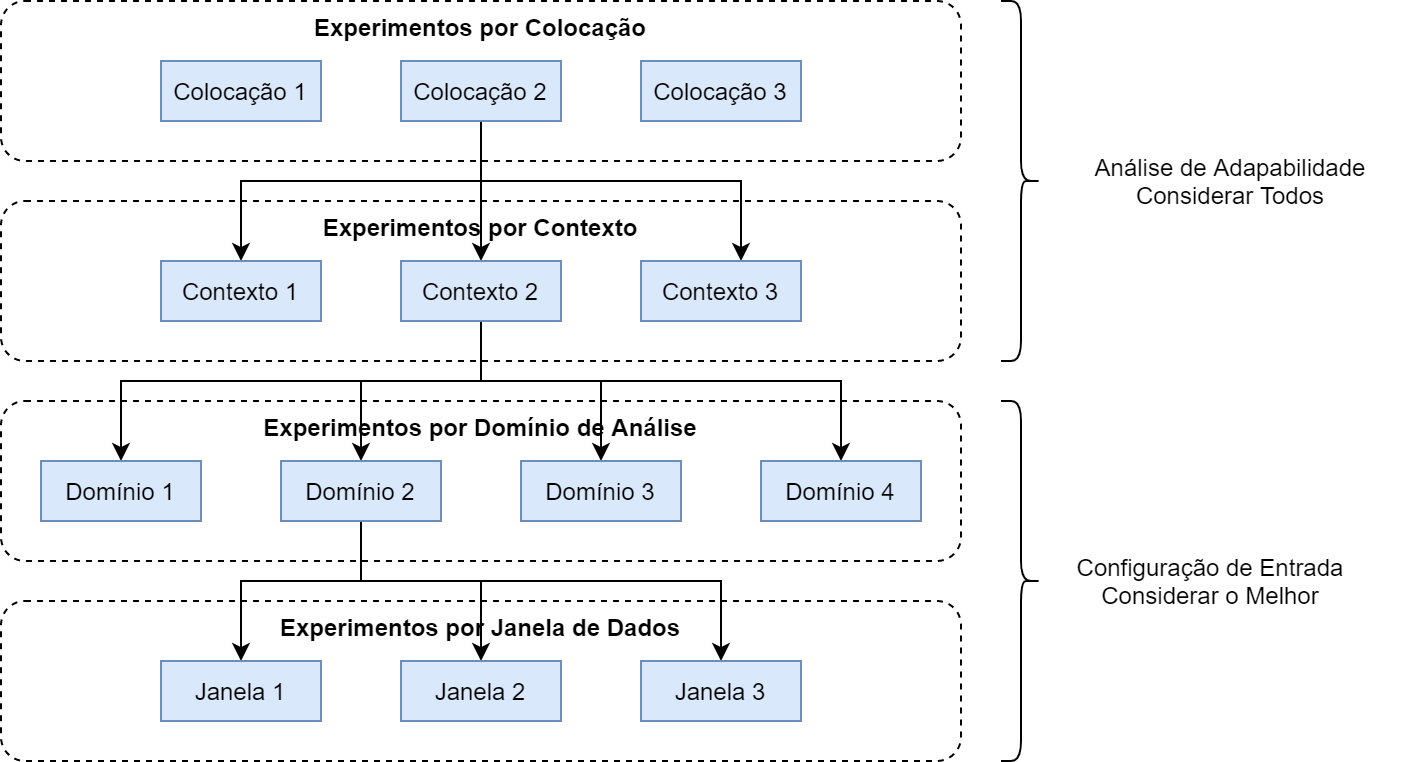
\includegraphics[width=1\textwidth]{figuras/fig_36_1.png}
 \fonte{Desenvolvido pelo autor.}
\end{figure}

\section{Processamento}

Após a etapa de pré-processamento, os dados foram aplicados em modelos de classificação baseados em \textit{Deep Learning}. Neste estudo, foram desenvolvidas DNN baseadas em LSTM, GRU e CNN. Todos os modelos são sequenciais e utilizam o otimizador Adam em conjunto com a função de perda de Entropia Cruzada Categórica. O modelo baseado em LSTM é ilustrado na \autoref{fig:best_lstm_tipo_superficie_2}, sendo composto por um bloco de camada de entrada, três blocos de camadas de recorrência e regularização e um bloco de camadas totalmente conectadas para produção de saída. O bloco de entrada possui uma camada que recebe um tensor \emph{janelas x sequências x características}, onde \emph{janelas} são os agrupamentos de janelas, \emph{sequências} são os dados que compõem uma das janelas e \emph{características} os valores das 7 variáveis. Cada bloco de recorrência e regularização é composto por uma camada LSTM unidirecional de 100 unidades, seguido por uma camada de \textit{Batch Normalization} e outra de \textit{Dropout} em 50\%. Após o processamento nas camadas recorrentes, os parâmetros passam para o bloco de camadas totalmente conectadas, onde existem duas camadas \textit{Dense}, a primeira com 100 neurônios com ativação \textit{Relu} e a segunda com 3 neurônios e ativação \textit{Softmax}, produzindo a classificação. A saída esperada da rede são os rótulos correspondentes à última amostra na janela. O modelo baseado em GRU desenvolvido possuí a mesma estrutura LSTM, trocando camadas LSTM por GRU conforme detalha a \autoref{fig:best_gru_tipo_superficie_2}.

\begin{figure}[h!]
  \centering
  \caption{Modelo LSTM para classificação do tipo de superfície de pista}
  \label{fig:best_lstm_tipo_superficie_2}
  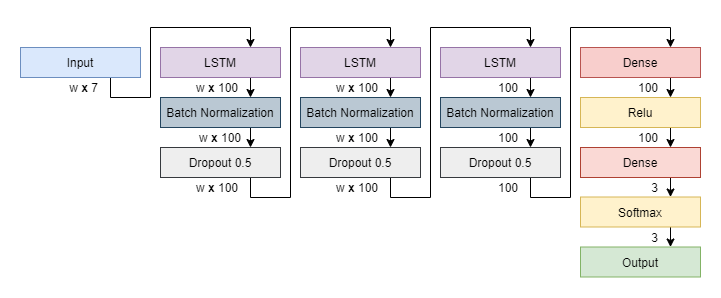
\includegraphics[width=0.8\textwidth]{figuras/fig_37.png}
 \fonte{Desenvolvido pelo autor.}
\end{figure}

\begin{figure}[h!]
  \centering
  \caption{Modelo GRU para classificação do tipo de superfície de pista}
  \label{fig:best_gru_tipo_superficie_2}
  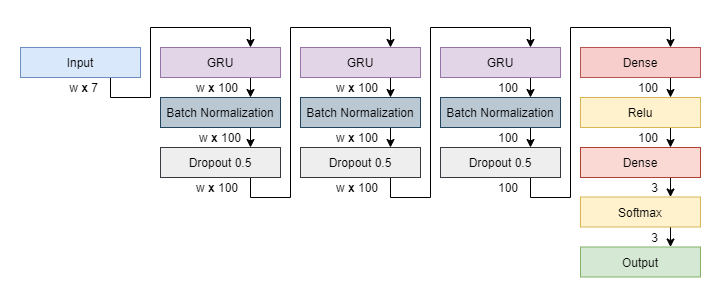
\includegraphics[width=0.8\textwidth]{figuras/fig_38.png}
 \fonte{Desenvolvido pelo autor.}
\end{figure}

\begin{figure}[h!]
  \centering
  \caption{Modelo CNN para classificação do tipo de superfície de pista}
  \label{fig:best_cnn_tipo_superficie_2}
  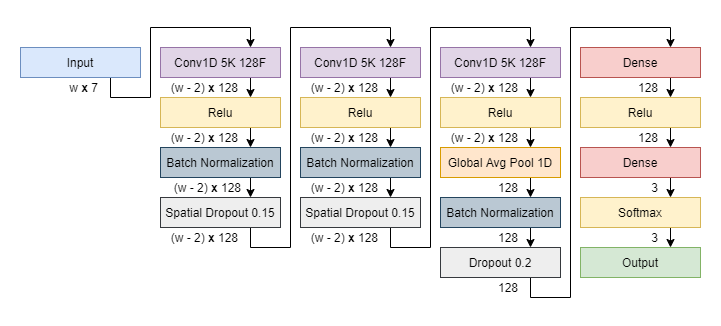
\includegraphics[width=0.8\textwidth]{figuras/fig_39.png}
 \fonte{Desenvolvido pelo autor.}
\end{figure}

Por fim, o modelo desenvolvido baseado em CNN é ilustrado na \autoref{fig:best_cnn_tipo_superficie_2}, sendo composto por um bloco de camada de entrada, três blocos de camadas de convolução e regularização e um bloco de camadas totalmente conectadas para produção de saída. O bloco de entrada possui uma camada que recebe um tensor \emph{janelas x sequências x características}, similar aos modelos LSTM e GRU. Os dois primeiros blocos de convolução e regularização são compostos cada um por uma camada Conv 1D com 128 filtros de \textit{kernel} tamanho 5 para extração de características e ativação \textit{Relu}, seguida por regularização através de uma camada de \textit{Batch Normalization} e outra de \textit{Spatial Dropout 1D} em 15\%. O último bloco de convolução e regularização possui uma camada Conv 1D com as mesmas configurações das anteriores, uma camada de \textit{Global Average Pooling 1D}, e camadas de regularização por \textit{Batch Normalization} e \textit{Dropout} em 20\%. Finalmente, o bloco de totalmente conectadas consiste em duas camadas \textit{Dense}, uma com 32 neurônios e ativação \textit{Relu} e outra com 3 neurônios e ativação \textit{Softmax}. A saída esperada da rede são os rótulos mais presentes na janela de dados.

Os demais hiperparâmetros das técnicas de \textit{Deep Learning} foram utilizados com seus valores padrões, disponíveis em \citeonline{tensorflow1}, \citeonline{tensorflow2} e \citeonline{tensorflow3}.

\section{Análise de Resultados}

Todos os modelos desenvolvidos neste estudo foram programados em Python 3, utilizando a biblioteca Keras do Tensorflow. Os experimentos foram realizados no Google \textit{Collaboratory}, em um ambiente com as mesmas configurações do estudo da seção anterior. Todas as configurações de treinamento estão detalhadas nos códigos-fonte documentados disponíveis na página do projeto no Github. Todos os experimentos foram executados três vezes, %a fim de minimizar a aleatoriedade dos parâmetros iniciais,
recuperando apenas o melhor modelo entre as três execuções. O melhor modelo foi considerado aquele que apresentou o maior valor de acurácia durante a validação. Os resultados obtidos foram agrupados por ponto de coleta de dados no veículo, detalhados nas Tabelas \ref{table:below_suspension_results_tipo_superficie_2}, \ref{table:above_suspension_results_tipo_superficie_2} e \ref{table:dashboard_results_tipo_superficie_2}. Além do agrupamento por ponto de coleta, em cada tabela é detalhado o experimento por modelo de DNN, domínio de análise, características de entrada e janelas de dados. Cada valor exibido corresponde a média de acurácia na validação dos três \emph{experimentos por contexto}, os quais visam analisar a capacidade de aprendizado e generalização do modelo para cenários não conhecidos, onde há variações contextuais correspondentes aos fatores de dependência veicular, de condução e ambientais. Os valores destacados correspondem ao valor máximo de média de acurácia em validação para dado tipo de DNN.

\begin{table}[h!]
\scriptsize
\centering
\caption{Média de acurácia para colocação próximo e abaixo da suspensão}
\label{table:below_suspension_results_tipo_superficie_2}
\begin{tabular}{cccccc}
\cmidrule(l){4-6} & \multicolumn{1}{l}{\textbf{}} & \multicolumn{1}{l}{} & \multicolumn{3}{c}{\textbf{Tamanho da Janela de Dados}} \\ \midrule
\textbf{Modelo} & \textbf{Domínio} & \textbf{Características} & \multicolumn{1}{c}{100} & \multicolumn{1}{c}{200} & \multicolumn{1}{c}{300} \\ \midrule
\multirow{5}{*}{LSTM} & \multirow{2}{*}{Tempo} 
& 7 & 89,69\% & 92,06\% & 92,34\% \\ \cmidrule(l){3-6} 
&  & 11 & 89,70\% & 90,99\% & 92,11\% \\ \cmidrule(l){2-6} 
& \multirow{2}{*}{Frequência} 
& 357 & 90,34\% & 91,86\% & 92,63\% \\ \cmidrule(l){3-6} 
&  & 561 & 90,65\% & 91,55\% & \cellcolor[HTML]{34FF34}92,82\% \\ \midrule
\multirow{5}{*}{GRU} & \multirow{2}{*}{Tempo} 
& 7 & 90,23\% & 92,06\% & \cellcolor[HTML]{34FF34}92,88\% \\ \cmidrule(l){3-6} 
&  & 11 & 89,81\% & 91,65\% & 92,31\% \\ \cmidrule(l){2-6} 
 & \multirow{2}{*}{Frequência} & 357 & 90,18\% & 91,09\% & 92,33\% \\ \cmidrule(l){3-6} 
 &  & 561 & 90,55\% & 91,59\% & 92,40\% \\ \midrule
\multirow{5}{*}{CNN} & \multirow{2}{*}{Tempo} & 7 & 91,16\% & 92,92\% & 93,04\% \\ \cmidrule(l){3-6} 
 &  & 11 & 90,24\% & 92,58\% & 92,60\% \\ \cmidrule(l){2-6} 
 & \multirow{2}{*}{Frequência} & 357 & 89,56\% & 91,92\% & \cellcolor[HTML]{34FF34}93,91\% \\ \cmidrule(l){3-6} 
 &  & 561 & 89,78\% & 92,08\% & 93,67\% \\ \bottomrule
\end{tabular}
\fonte{Desenvolvido pelo autor.}
\end{table}

\begin{table}[h!]
\scriptsize
\centering
\caption{Média de acurácia para colocação próximo e acima da suspensão}
\label{table:above_suspension_results_tipo_superficie_2}
\begin{tabular}{cccccc}
\cmidrule(l){4-6}
 & \multicolumn{1}{l}{\textbf{}} & \multicolumn{1}{l}{} & \multicolumn{3}{c}{\textbf{Tamanho da Janela de Dados}} \\ \midrule
\textbf{Modelo} & \textbf{Domínio} & \textbf{Características} & \multicolumn{1}{c}{100} & \multicolumn{1}{c}{200} & \multicolumn{1}{c}{300} \\ \midrule
\multirow{5}{*}{LSTM} & \multirow{2}{*}{Tempo} & 7 & 89,23\% & 90,56\% & \cellcolor[HTML]{34FF34}90,89\% \\ \cmidrule(l){3-6} 
 &  & 11 & 87,56\% & 88,96\% & 90,58\% \\ \cmidrule(l){2-6} 
 & \multirow{2}{*}{Frequência} & 357 & 88,41\% & 89,55\% & 90,78\% \\ \cmidrule(l){3-6} 
 &  & 561 & 88,04\% & 90,00\% & 90,15\% \\ \midrule
\multirow{5}{*}{GRU} & \multirow{2}{*}{Tempo} & 7 & 87,53\% & 89,16\% & 89,42\% \\ \cmidrule(l){3-6} 
 &  & 11 & 87,54\% & 88,61\% & 89,79\% \\ \cmidrule(l){2-6} 
 & \multirow{2}{*}{Frequência} & 357 & 88,57\% & 89,49\% & \cellcolor[HTML]{34FF34}90,41\% \\ \cmidrule(l){3-6} 
 &  & 561 & 87,84\% & 89,76\% & 90,05\% \\ \midrule
\multirow{5}{*}{CNN} & \multirow{2}{*}{Tempo} & 7 & 88,65\% & 90,85\% & \cellcolor[HTML]{34FF34}92,02\% \\ \cmidrule(l){3-6} 
 &  & 11 & 88,25\% & 90,04\% & 90,74\% \\ \cmidrule(l){2-6} 
 & \multirow{2}{*}{Frequência} & 357 & 88,32\% & 90,75\% & 91,01\% \\ \cmidrule(l){3-6} 
 &  & 561 & 88,23\% & 90,67\% & 90,92\% \\ \bottomrule
\end{tabular}
\fonte{Desenvolvido pelo autor.}
\end{table}

\begin{table}[h!]
\scriptsize
\centering
\caption{Média de acurácia para colocação no painel de controle}
\label{table:dashboard_results_tipo_superficie_2}
\begin{tabular}{cccccc}
\cmidrule(l){4-6}
 & \multicolumn{1}{l}{\textbf{}} & \multicolumn{1}{l}{} & \multicolumn{3}{c}{\textbf{Tamanho da Janela de Dados}} \\ \midrule
\textbf{Modelo} & \textbf{Domínio} & \textbf{Características} & 100 & 200 & \multicolumn{1}{c}{300} \\ \midrule
\multirow{5}{*}{LSTM} & \multirow{2}{*}{Tempo} & 7 & 89,64\% & \cellcolor[HTML]{34FF34}91,79\% & 91,64\% \\ \cmidrule(l){3-6} 
 &  & 11 & 88,54\% & 90,96\% & 91,73\% \\ \cmidrule(l){2-6} 
 & \multirow{2}{*}{Frequência} & 357 & 88,61\% & 89,47\% & 90,92\% \\ \cmidrule(l){3-6} 
 &  & 561 & 89,90\% & 91,03\% & 91,55\% \\ \midrule
\multirow{5}{*}{GRU} & \multirow{2}{*}{Tempo} & 7 & 89,82\% & 91,67\% & \cellcolor[HTML]{34FF34}91,91\% \\ \cmidrule(l){3-6} 
 &  & 11 & 89,62\% & 90,83\% & 91,73\% \\ \cmidrule(l){2-6} 
 & \multirow{2}{*}{Frequência} & 357 & 88,76\% & 90,53\% & 90,74\% \\ \cmidrule(l){3-6} 
 &  & 561 & 89,67\% & 90,92\% & 91,68\% \\ \midrule
\multirow{5}{*}{CNN} & \multirow{2}{*}{Tempo} & 7 & 89,44\% & 91,46\% & 93,05\% \\ \cmidrule(l){3-6} 
 &  & 11 & 89,64\% & 91,50\% & 93,30\% \\ \cmidrule(l){2-6} 
 & \multirow{2}{*}{Frequência} & 357 & 89,40\% & 91,51\% & 92,37\% \\ \cmidrule(l){3-6} 
 &  & 561 & 89,70\% & 92,09\% & \cellcolor[HTML]{34FF34}93,57\% \\ \bottomrule
\end{tabular}
\fonte{Desenvolvido pelo autor.}
\end{table}


Através das tabelas de resultados, é possível observar que o tamanho da janela de dados pouco influencia o resultado final. Considerando todos os experimentos realizados, o aumento da janela de dados de 100 para 200 amostras aumentou em média cerca de 1,8\% a média de acurácia em validação, enquanto que o aumento de 200 amostras para 300 acrescentou cerca de 0,8\%. Em relação a utilização das variáveis brutas dos sensores (7 características) e a magnitude de suas frequências (357 características) quando comparadas a adição das variáveis de aceleração composta (11 características) e a magnitude das frequências (561 características) foi observado uma variação média de 0,1\% no valor de acurácia, sendo que em 54\% dos melhores experimentos não utilizaram da aceleração composta, e outros 46\% utilizaram. De maneira geral, a adição destas variáveis não se justifica, aumentando o custo computacional sem ter um aumento consistente de acurácia.

Em relação aos domínios de análise, tanto o domínio do tempo quanto o domínio da frequência obtiveram bons resultados. Quando comparados os experimentos com as variáveis no domínio do tempo com sua respectiva representação no domínio da frequência, metade dos experimentos foi melhor no domínio do tempo e a outra metade teve melhor desempenho no domínio da frequência. Contudo, a variação média de acurácia entre os domínios de análise é de apenas 0,05\% e, considerando o custo de transformação entre domínios e o aumento expressivo de características de entrada quando representadas no domínio da frequência, passando de 7 no domínio do tempo para 357 com sua representação na frequência, e de 11 no domínio do tempo para 561 com sua representação na frequência, o domínio do tempo mostra-se mais adequado.

Analisando os modelos de DNN propostos, observamos que todos obtiveram bons resultados, com pouca variação de resultados. Considerando todos os experimentos, a rede baseada em CNN obteve melhores resultados, seguida pela LSTM e pela GRU. Contudo, a variação média dos valores de acurácia entre os três modelos é menor que 1\%. Em relação aos diferentes pontos de coleta no veículo, observamos que as redes são capazes de classificar corretamente mesmo com interferência da dependência veicular. Em uma análise ampla, as redes têm mais facilidade em reconhecer os padrões dos dados amostrados próximo abaixo da suspensão, seguidos pelos amostrados no painel de controle e por fim os amostrados próximo e acima da suspensão. Contudo, a variação média de acurácia entre os pontos de coleta é pequena, cerca de 2\%.

Em uma análise macro de todos os experimentos, observamos que as redes propostas nas suas diversas variações de configuração de dados de entrada realizam a classificação de superfície de pista com bons valores de acurácia em validação, validando a hipótese deste estudo e evidenciando a capacidade das redes de \textit{Deep Learning} aprenderem as relações dos dados com as propriedades de dependência, generalizando para cenários desconhecidos. Com base em todas as análises individuais realizadas, consideramos o melhor modelo de classificação de pista o modelo baseado em CNN, processando no domínio do tempo 7 características correspondentes aos dados brutos dos sensores, em uma janela de dados de 300 amostras. A Tabela \ref{table:cnn_results_tipo_superficie_2} detalha os valores de acurácia em treinamento e validação do modelo CNN para cada \emph{experimento por contexto} e \emph{experimento por colocação}. A \autoref{table:cnn_metrics_tipo_superficie_2} detalha as demais métricas de avaliação e a \autoref{fig:cnn_confusion_matrix_tipo_superficie_2} detalha as matrizes de confusão correspondentes.

\begin{table}[h!]
\scriptsize
\centering
\caption{Valores de acurácia para o modelo baseado em CNN}
\label{table:cnn_results_tipo_superficie_2}
\begin{tabular}{cccccc}
\toprule
\multirow{2}{*}{\textbf{\begin{tabular}[c]{@{}c@{}}Experimento \\ por Colocação\end{tabular}}} & \multirow{2}{*}{\textbf{\begin{tabular}[c]{@{}c@{}}Fase de \\ Processamento\end{tabular}}} & \multicolumn{4}{c}{\textbf{Experimento por Contexto}} \\ \cmidrule(l){3-6} 
 &  & 1 & 2 & 3 & Média \\ \midrule
\multirow{2}{*}{\begin{tabular}[c]{@{}c@{}}Próximo e abaixo \\ da suspensão\end{tabular}} & Treinamento & 94,67\% & 94,40\% & 97,01\% & 95,36\% \\ \cmidrule(l){2-6} 
 & Validação & 94,78\% & 92,17\% & 92,17\% & 93,04\% \\ \midrule
\multirow{2}{*}{\begin{tabular}[c]{@{}c@{}}Próximo e acima\\ da suspensão\end{tabular}} & Treinamento & 88,46\% & 92,89\% & 95,45\% & 92,27\% \\ \cmidrule(l){2-6} 
 & Validação & 94,11\% & 90,14\% & 91,80\% & 92,02\% \\ \midrule
\multirow{2}{*}{Painel de Controle} & Treinamento & 93,16\% & 94,84\% & 97,50\% & 95,17\% \\ \cmidrule(l){2-6} 
 & Validação & 95,25\% & 89,93\% & 93,96\% & 93,05\% \\ \bottomrule
\end{tabular}
\fonte{Desenvolvido pelo autor.}
\end{table}

\begin{table}[h!]
\scriptsize
\centering
\caption{Métricas de avaliação para o modelo baseado em CNN}
\label{table:cnn_metrics_tipo_superficie_2}
\begin{tabular}{clccc}
\toprule
\textbf{Colocação} & \multicolumn{1}{c}{\textbf{Classe de Dados}} & \textbf{F1-Score} & \textbf{Precisão} & \textbf{Recall} \\ \midrule
\multirow{4}{*}{\begin{tabular}[c]{@{}c@{}}Próximo e abaixo\\ da suspensão\end{tabular}} & Asfalto & 98,60\% & 98,59\% & 98,62\% \\ \cmidrule(l){2-5} 
 & Paralelepípedo & 86,09\% & 88,39\% & 83,90\% \\ \cmidrule(l){2-5} 
 & Terra & 90,78\% & 89,22\% & 92,39\% \\ \midrule
\multirow{4}{*}{\begin{tabular}[c]{@{}c@{}}Próximo e acima\\ da suspensão\end{tabular}} & Asfalto & 98,76\% & 99,08\% & 98,43\% \\ \cmidrule(l){2-5} 
 & Paralelepípedo & 84,18\% & 83,49\% & 84,87\% \\ \cmidrule(l){2-5} 
 & Terra & 89,06\% & 89,20\% & 88,91\% \\ \midrule
\multirow{4}{*}{Painel de Controle} & Asfalto & 98,62\% & 98,23\% & 99,02\% \\ \cmidrule(l){2-5} 
 & Paralelepípedo & 85,47\% & 90,13\% & 81,27\% \\ \cmidrule(l){2-5} 
 & Terra & 91,12\% & 88,58\% & 93,81\% \\ \bottomrule
\end{tabular}
\fonte{Desenvolvido pelo autor.}
\end{table}

\begin{figure}[h!]
  \centering
  \caption{Matriz de confusão para o modelo de CNN em cada ponto de coleta de dados}
  \label{fig:cnn_confusion_matrix_tipo_superficie_2}
  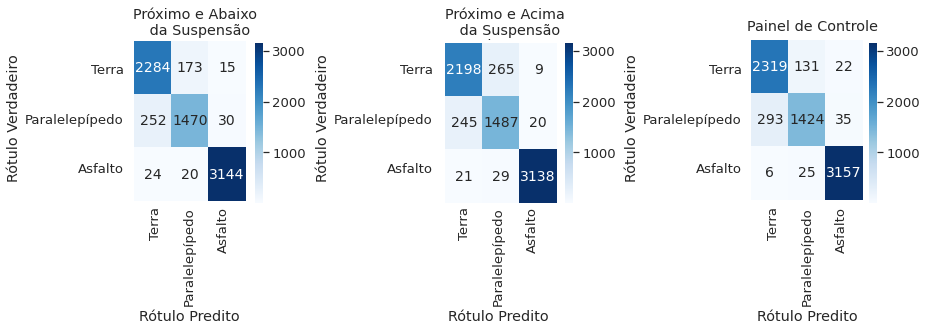
\includegraphics[width=1\textwidth]{figuras/fig_36.png}
  \fonte{Desenvolvido pelo autor.}
\end{figure}

Através das Tabelas \ref{table:cnn_results_tipo_superficie_2} e \ref{table:cnn_metrics_tipo_superficie_2}, e da \autoref{fig:cnn_confusion_matrix_tipo_superficie_2} observamos que a rede CNN demonstrou boa capacidade de aprendizado e generalização para todos os pontos de coleta e todas as variações de contexto. Para os dados amostrados próximo e abaixo da suspensão, a rede obteve média de acurácia de treinamento de 95,36\% e de 93,04\% em validação, classificando segmentos de asfalto com \textit{f1-score} de 98,60\%, paralelepípedo com 86,09\% e terra com 90,78\%. Para os dados amostrados próximo e acima da suspensão, o modelo obteve média de acurácia em treinamento de 92,27\% e de 92,02\% em validação, classificando segmentos de asfalto com \textit{f1-score} de 98,76\%, paralelepípedo com 84,18\% e terra com 86,06\%. Por fim, para os dados amostrados no painel de controle obteve-se média de acurácia em treinamento de 95,17\% e de 93,05\% em validação, classificando segmentos de asfalto com \textit{f1-score} de 98,62\%, paralelepípedo com 85,47\% e terra com 91,12\%. Observa-se que os resultados obtidos são superiores aos estudos anteriores, adicionando-se que neste estudo a análise foi realizada em contextos com variações das propriedades de dependência.